%=================================================================
% This template is based on IMRT Latex template by Eric A. Mueller
%================================================================= 

\documentclass[10pt,twoside,a4paper]{report}

 \usepackage[bt,fs,english]{ethasl}   % New styles and commands
                                      % Options: 	bt/mt: Bachelorthesis/Masterthesis
                                      %						fs/hs: Fr�hlingssemester/Herbstsemester
                                      %						german/english: Deutsch/English

% \includeonly{}                      % Quick formatting
% \usepackage[draft]{graphicx}        % Quick formatting

 \usepackage{a4}                      % Paper size
 \usepackage[latin1]{inputenc}        % Keybord settings
 \usepackage{amsmath}                 % Additional math functionality
 \usepackage{amssymb}                 % Additional math functionality
 \usepackage{graphicx}                % EPS figures
 \usepackage[dvips]{epsfig}           % EPS figures
 \usepackage{float}                   % Placement of floating objects
 \usepackage{fancyhdr}                % Headings
 \usepackage{rotating}
 \usepackage{multirow}
 \usepackage{url}
 \usepackage{colortbl}
 \usepackage{ifpdf}
 

 \usepackage{hyperref}
 \usepackage{color}
 \definecolor{black}{rgb}{0,0,0}
 \definecolor{white}{rgb}{1,1,1}

 \definecolor{darkred}{rgb}{0.5,0,0}
 \definecolor{darkgreen}{rgb}{0,0.5,0}
 \definecolor{darkblue}{rgb}{0,0,0.5}

 \hypersetup{colorlinks
	,linkcolor=black
	,filecolor=black
	,urlcolor=black
	,citecolor=black
 }


 \ifpdf
	\usepackage[update]{epstopdf}
 \else
 \fi

 \usepackage{german}                  % German language "o, "a, use.
%\usepackage{ae}                      % German specials

%---------------------------------------------------------------------------

 \setlength{\parindent}{0em}                   % Disable parindent
 \rhead[\thepage]{\nouppercase{\rightmark}}    % Special headings
 \lhead[\nouppercase{\leftmark}]{\thepage}     % Special headings
 \cfoot{}                                      % Special headings

%---------------------------------------------------------------------------

 \title{Human-Machine Interface for Operating a Blimb}
 %\subtitle{bla bla bla}

 
 \studentA{Krebs Matthias}
 \studentB{Ledergerber Anton}
% \studentC{Student 3}
 
 

\supervisionA{Konrad Rudin}
\supervisionB{Mora Javier Alonso}
\supervisionC{Paul Beardsley XXXXX}
 

%===========================================================================
\begin{document}

%---------------------------------------------------------------------------
% Title page

 \maketitle
 \pagestyle{plain}
 \pagenumbering{roman}

%---------------------------------------------------------------------------
% Declaration of Originality

\pagestyle{empty}
% TODO Modify placeholders in declaration.tex
%---------------------------------------------------------------------------
% Declaration of Originality
%
% TODO Add title, student first/last name, supervisor first/last name.

\section*{Declaration of Originality}

\vspace{1cm}

I hereby declare that the written work I have submitted entitled

\vspace{0.5cm}

% TODO Add title
\textbf{Bio-Inspired, Solar-Powered, Autonomous Flapping Wing Micro Aerial Vehicle}

\vspace{0.5cm}

is original work which I alone have authored and which is written in my own words.\footnote{Co-authored work: The signatures of all authors are required. Each signature attests to the originality of the entire piece of written work in its final form.}

\vspace{1cm}

\textbf{Author(s)}

\vspace{0.5cm}

\begin{tabular}{ p{5cm} p{5cm} }
% TODO Add student first/last name
  Anton & Ledergerber \\
  Matthias & Krebs \\
\end{tabular}

\vspace{0.5cm}

\textbf{Supervising lecturer}

\vspace{0.5cm}

\begin{tabular}{ p{5cm} p{5cm} }
% TODO Add supervisor first/last name
  Konrad & Rudin \\
  Javier Alonso & Mora \\
  Paul XXX & Beardsley XXX \\
\end{tabular}

\vspace{1cm}

With the signature I declare that I have been informed regarding normal academic citation rules and that I have read and understood the information on 'Citation etiquette' (\url{http://www.ethz.ch/students/exams/plagiarism_s_en.pdf}). The citation conventions usual to the discipline in question here have been respected.

\vspace{0.5cm}

The above written work may be tested electronically for plagiarism.

\vspace{4cm}

\begin{tabular}{ p{5cm} p{1cm} p{5cm} }
  \cline{1-1} \cline{3-3}
  Place and date & & Signature \\
\end{tabular}

%---------------------------------------------------------------------------



%---------------------------------------------------------------------------
% Preamble

 %---------------------------------------------------------------------------
% Preface

%\chapter*{Vorwort}

%Bla bla \dots

 %\cleardoublepage

%---------------------------------------------------------------------------
% Table of contents

 \setcounter{tocdepth}{2}
 \tableofcontents

 \cleardoublepage

%---------------------------------------------------------------------------
% Abstract

%\chapter*{Zusammenfassung}
% \addcontentsline{toc}{chapter}{Zusammenfassung}

%Bla bla \dots

% \cleardoublepage

\chapter*{Abstract}
 \addcontentsline{toc}{chapter}{Abstract}

Hier kommt der Abstact hin \dots

 \cleardoublepage

%---------------------------------------------------------------------------
% Acknowledgements

%\chapter*{Acknowledgements}\label{chap:Acknowledgements}
% \addcontentsline{toc}{chapter}{Acknowledgements}
\chapter*{Acknowledgements}
 \addcontentsline{toc}{chapter}{Acknowledgements}

Without the help of a few people this thesis would not have been possible. We received the necessary support from all sides throughout the project to realize the this HMI which we are proud of.

Prof. Dr. Roland Y. Siegwart\\
Dr. Paul Beardsley\\
Phd students Konrad Rudin and Javier Alonso Mora\\
Gerhard R"othlin\\
Lorentz Meier\\
Alexander Rudyk\\



 \cleardoublepage

%---------------------------------------------------------------------------
% Symbols

%\chapter*{Symbolverzeichnis}\label{chap:symbole}
% \addcontentsline{toc}{chapter}{Symbolverzeichnis}
\chapter*{Symbols}\label{chap:symbole}
 \addcontentsline{toc}{chapter}{Symbols}

%\section*{Symbole}
\section*{Symbols}
\begin{tabbing}
 \hspace*{3cm} \= \kill
  $\phi, \theta, \psi$ 					\> roll, pitch and yaw angle \\[0.5ex] 					
  $b$														\> gyroscope bias \\[0.5ex]										
  $\Omega_m$										\> 3-axis gyroscope measurement \\[0.5ex]   		
 \end{tabbing}

%\section*{Indizes}
\section*{Indices}
\begin{tabbing}
 \hspace*{1.6cm}  \= \kill
 $x$ \> x axis \\[0.5ex]
 $y$ \> y axis \\[0.5ex]
 
\end{tabbing}

%\section*{Akronyme und Abk�rzungen}
\section*{Acronyms and Abbreviations}
\begin{tabbing}
 \hspace*{1.6cm}  \= \kill
 ETH \> Eidgen�ssische Technische Hochschule \\[0.5ex]
 EKF \> Extended Kalman Filter \\[0.5ex]
 IMU \> Inertial Measurement Unit \\[0.5ex]
 UAV \> Unmanned Aerial Vehicle \\[0.5ex]
 UKF \> Unscented Kalman Filter \\[0.5ex]
\end{tabbing}

 \cleardoublepage

%---------------------------------------------------------------------------


 \pagestyle{headings}                 % Default headings
 \pagestyle{fancy}                   % Special headings
 \pagenumbering{arabic}

%---------------------------------------------------------------------------
% Chapters

 \chapter{Introduction}\label{sec:introduction}

%\section{Motivation}

\section{Context}

\section{Goals}

\section{System Overview}

\section{Similar Systems and their HMI}

\section{Structure of the Report}
 \cleardoublepage
 
\chapter{Einige wichtige Hinweise zum Arbeiten mit \LaTeX\ }\label{sec:latexumg}

Nachfolgend wird die Codierung einiger oft verwendeten Elemente
kurz beschrieben. Das Einbinden von Bildern ist in \LaTeX\ nicht
ganz unproblematisch und h�ngt auch stark vom verwendeten Compiler
ab. Typisches Format f�r Bilder in \LaTeX\ ist
EPS\footnote{Encapsulated Postscript}.


\section{Gliederungen}\label{sec:gliederung}

Ein Text kann mit den Befehlen \texttt{\textbackslash
chapter\{.\}}, \texttt{\textbackslash section\{.\}},
\texttt{\textbackslash subsection\{.\}} und \texttt{\textbackslash
subsubsection\{.\}} gegliedert werden.


\section{Referenzen und Verweise}\label{sec:refverw}

Literaturreferenzen werden mit dem Befehl \texttt{\textbackslash
cite\{.\}} erzeugt. Ein Beispiel: \cite{optreg}.

Zur Erzeugung von Fussnoten wird der Befehl \texttt{\textbackslash
footnote\{.\}} verwendet. Auch hier ein Beispiel\footnote{Bla
bla.}.

Querverweise im Text werden mit \texttt{\textbackslash label\{.\}}
verankert und mit \texttt{\textbackslash ref\{.\}} erzeugt.
Beispiel einer Referenz auf das zweite Kapitel:
Kapitel~\ref{sec:latexumg}.


\section{Aufz�hlungen}\label{sec:aufz}

Folgendes Beispiel einer Aufz�hlung ohne Numerierung,
\begin{itemize}
  \item Punkt 1
  \item Punkt 2
\end{itemize}
wurde erzeugt mit:
\begin{verbatim}
\begin{itemize}
  \item Punkt 1
  \item Punkt 2
\end{itemize}
\end{verbatim}

Folgendes Beispiel einer Aufz�hlung mit Numerierung,
\begin{enumerate}
  \item Punkt 1
  \item Punkt 2
\end{enumerate}
wurde erzeugt mit:
\begin{verbatim}
\begin{enumerate}
  \item Punkt 1
  \item Punkt 2
\end{enumerate}
\end{verbatim}

Folgendes Beispiel einer Auflistung,
\begin{description}
  \item[P1] Punkt 1
  \item[P2] Punkt 2
\end{description}
wurde erzeugt mit:
\begin{verbatim}
\begin{description}
  \item[P1] Punkt 1
  \item[P2] Punkt 2
\end{description}
\end{verbatim}


\section{Erstellen einer Tabelle}\label{sec:tabellen}

Ein Beispiel einer Tabelle:
\begin{table}[h]
\begin{center}
 \caption{Daten der Fahrzyklen ECE, EUDC, NEFZ.}\vspace{1ex}
 \label{tab:tabnefz}
 \begin{tabular}{ll|ccc}
 \hline
 Kennzahl & Einheit & ECE & EUDC & NEFZ \\ \hline \hline
 Dauer & s & 780 & 400 & 1180 \\
 Distanz & km & 4.052 & 6.955 & 11.007 \\
 Durchschnittsgeschwindigkeit & km/h & 18.7 &  62.6 & 33.6 \\
 Leerlaufanteil & \% & 36 & 10 & 27 \\
 \hline
 \end{tabular}
\end{center}
\end{table}

Die Tabelle wurde erzeugt mit:
\begin{verbatim}
\begin{table}[h]
\begin{center}
 \caption{Daten der Fahrzyklen ECE, EUDC, NEFZ.}\vspace{1ex}
 \label{tab:tabnefz}
 \begin{tabular}{ll|ccc}
 \hline
 Kennzahl & Einheit & ECE & EUDC & NEFZ \\ \hline \hline
 Dauer & s & 780 & 400 & 1180 \\
 Distanz & km & 4.052 & 6.955 & 11.007 \\
 Durchschnittsgeschwindigkeit & km/h & 18.7 &  62.6 & 33.6 \\
 Leerlaufanteil & \% & 36 & 10 & 27 \\
 \hline
 \end{tabular}
\end{center}
\end{table}
\end{verbatim}


\section{Einbinden einer EPS-Graphik}\label{sec:epsgraph}

Das Einbinden von Graphiken kann wie folgt bewerkstelligt werden:
\begin{verbatim}
\begin{figure}[h]
   \centering
   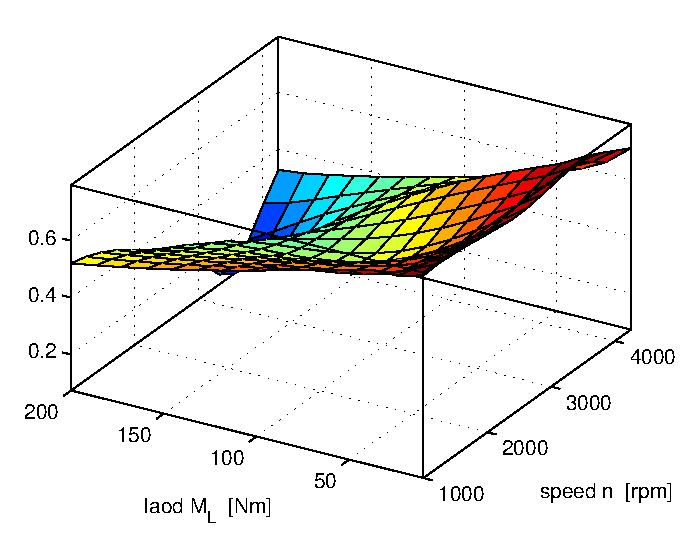
\includegraphics[width=0.75\textwidth]{pics/k_surf.eps}
   \caption{Ein Bild.}
   \label{pics:k_surf}
\end{figure}
\end{verbatim}

\begin{figure}[h]
   \centering
   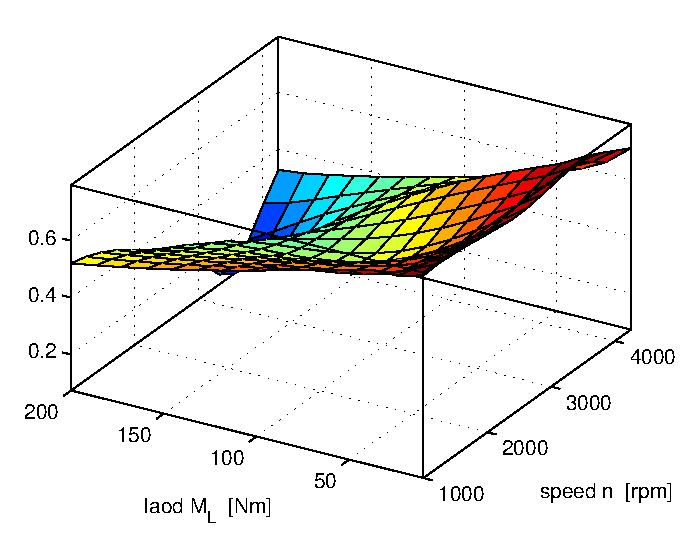
\includegraphics[width=0.75\textwidth]{pics/k_surf.eps}
   \caption{Ein Bild.}
   \label{pics:k_surf}
\end{figure}

oder bei zwei Bildern nebeneinander mit:
\begin{verbatim}
\begin{figure}[h]
  \begin{minipage}[t]{0.48\textwidth}
    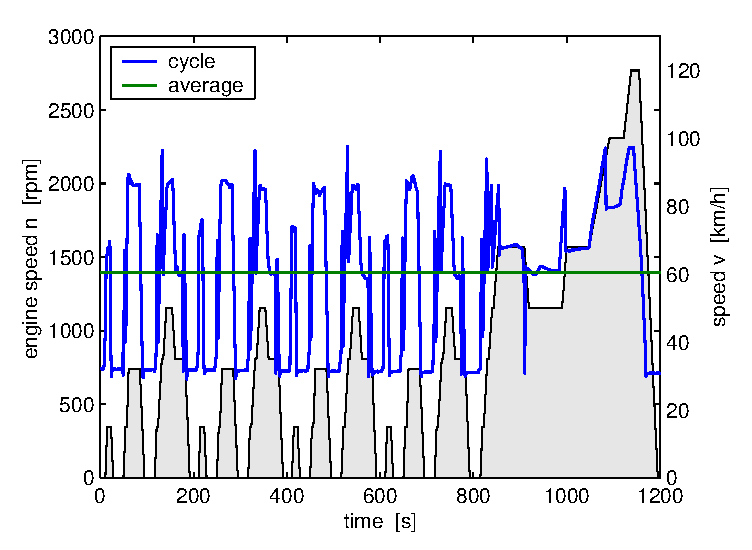
\includegraphics[width = \textwidth]{pics/cycle_we.eps}
  \end{minipage}
  \hfill
  \begin{minipage}[t]{0.48\textwidth}
    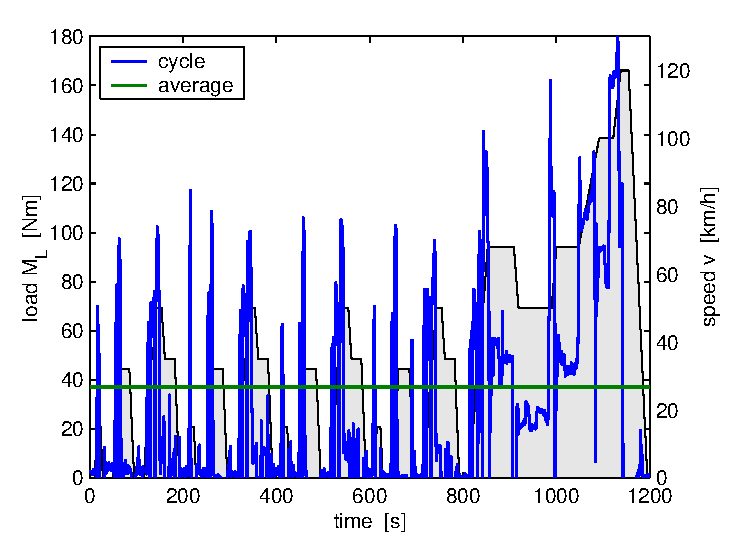
\includegraphics[width = \textwidth]{pics/cycle_ml.eps}
  \end{minipage}
  \caption{Zwei Bilder nebeneinander.}
  \label{pics:cycle}
\end{figure}
\end{verbatim}

\begin{figure}[h]
  \begin{minipage}[t]{0.48\textwidth}
    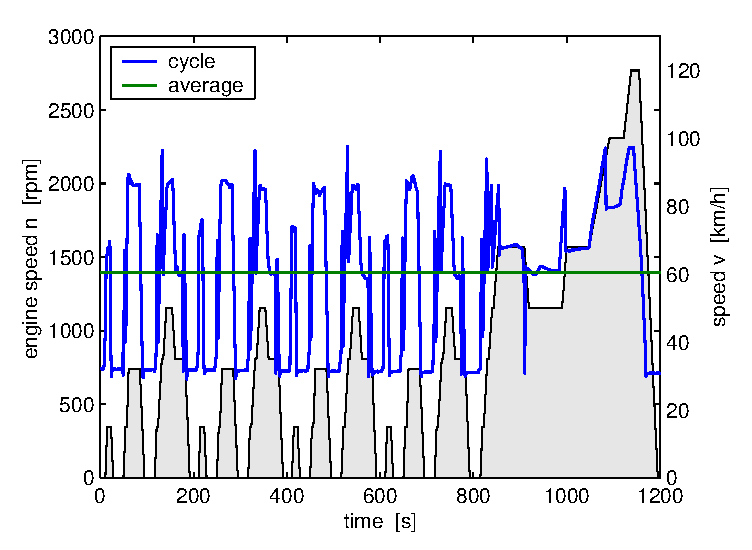
\includegraphics[width = \textwidth]{pics/cycle_we.eps}
  \end{minipage}
  \hfill
  \begin{minipage}[t]{0.48\textwidth}
    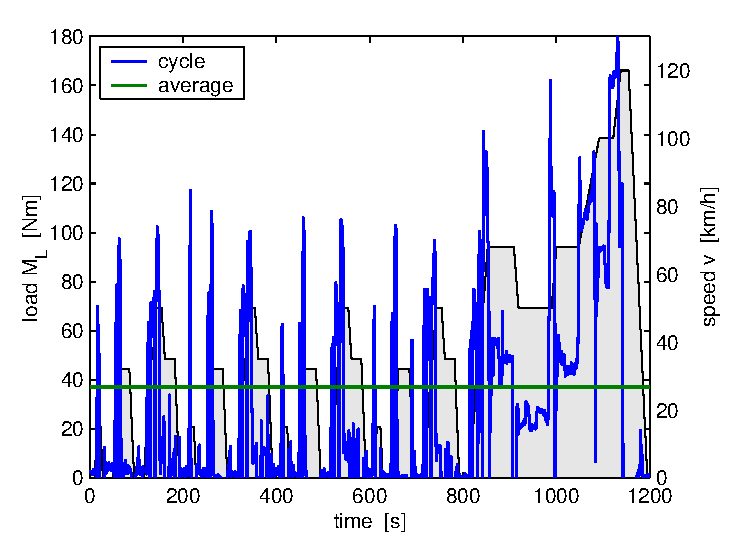
\includegraphics[width = \textwidth]{pics/cycle_ml.eps}
  \end{minipage}
  \caption{Zwei Bilder nebeneinander.}
  \label{pics:cycle}
\end{figure}

Bemerkung: Ersetzt man den Positionierungsparameter \texttt{h}
durch \texttt{H}, so wird das Gleiten der Abbildung verhindert.


\section{Mathematische Formeln}\label{sec:math}

Einfache mathematische Formeln werden mit der equation-Umgebung
erzeugt:
\begin{equation}
 p_{me0f}(T_e,\omega_e) \ = \ k_1(T_e) \cdot (k_2+k_3 S^2
 \omega_e^2) \cdot \Pi_{max} \cdot \sqrt{\frac{k_4}{B}} \, .
\end{equation}

Der Code dazu lautet:
\begin{verbatim}
\begin{equation}
 p_{me0f}(T_e,\omega_e) \ = \ k_1(T_e) \cdot (k_2+k_3 S^2
 \omega_e^2) \cdot \Pi_{max} \cdot \sqrt{\frac{k_4}{B}} \, .
\end{equation}
\end{verbatim}

Mathematische Ausdr�cke im Text werden mit \$formel\$ erzeugt (zB:
$a^2+b^2=c^2$).


\section{Weitere n�tzliche Befehle}\label{sec:div}

Hervorhebungen im Text sehen so aus: \emph{hervorgehoben}. Erzeugt
werden sie mit dem \texttt{\textbackslash epmh\{.\}} Befehl.

 \cleardoublepage
 
\chapter{Finding a Hardware and Software Solution}
 \cleardoublepage
 
\chapter{The different Control Modes}
 \cleardoublepage
 
\chapter{Realization of the HMI as a whole and for each Control Mode}
 \cleardoublepage
 \chapter{Trajectory Planning}
For the two most advanced modes, i. e. the Half-Automatic and the Full-Automatic Mode, trajectories had to be generated. In this chapter the best trajectories for skye are elaborated.

\section{Introduction}

\subsection{Definition}
What is a trajectory...(notation, parameter, time...)
How do we intend to realize our idea... 

\subsection{Our approach}
From the GUI it was given that the goal trajectory would be a multipoint-interpolating trajectory. The user is able to define waypoints on a map which afterwards should be connected with a reasonable and realizable trajectory. Beside interpolating trajectories there exist also approximating trajectories but they were not taken into consideration, since usually the user wants skye fly directly through a waypoint.

In another Bsc Thesis elaborated in this project a controller for waypoint following was designed. So it was convenient in the scope of this Thesis to use this controller instead of a specialized trajectory controller.

\section{Constraints from the system on the trajectory}

\subsection{Maximum velocities and accelerations}
In order to plan a feasible trajectory one has to know the capabilities of the system. Here just a basic derivation for the velocities and accelerations is given, for more details refer to (!!!!Bsc Thesis Joe, Bsc Thesis Andy)\\

The maximum feasible acceleration in any direction is calculated to be:

\begin{equation}
  \left|a_{max} \right| =  \frac{\left|F_{res, w}\right|}{m_{tot}} = 0.96 m/s^2
\end{equation}

Whereas the $F_{res,w}$ is the force resulting from all four thrusters operated under full load in the worst direction and $m_{tot}$ is the sum of the masses of the helium, the virtual mass and the mass of the system itself.\\


The maximum feasible velocity in any direction is calculated to be:

\begin{equation}
\left|v_{max} \right| = \sqrt{\frac{\left|F_{res,w} \right|}{\frac{1}{2}c_d \rho \pi r^2}}=4.7 m/s
\end{equation}

which is nothing but $ \left|F_{res,min} \right| = \left|F_{dray} \right| $.\\

For trajectories for position and orientation the maximal feasible angular acceleration is also important. It is calculated to be:

\begin{equation}
  \left|\Psi_{max} \right| =  \frac{\left|M_{res,w}\right|}{\left| \lambda_{max, J_{B}} \right|} = 2.82 rad/s^2 
\end{equation}

which is quite conservative because it is assumed that worst axis for turning is also the principle axis of the inertia tensor with the highest inertia.\\

Since the system is almost undamped for rotations, the rotational velocities will never be the limiting factor.





\subsection{Continuity}








 \cleardoublepage
% ...
%
%---------------------------------------------------------------------------
% Appendix

 \appendix
 
\chapter{Irgendwas}\label{sec:irgendwas}

Bla bla \dots

 \cleardoublepage


\chapter{Nochmals irgendwas}\label{sec:nochirgendwas}

Bla bla \dots

 \cleardoublepage

%
%---------------------------------------------------------------------------
% Literature

 
\begin{thebibliography}{99}
%\addcontentsline{toc}{chapter}{Literaturverzeichnis}
\addcontentsline{toc}{chapter}{Bibliography}



\bibitem {comfilt} {\sc R.~Mahony, T.~Hamel, J.-M.~Pflimlin}:
{\it Complementary filter design on the special orthogonal group SO(3)}. In 45th Conference
on Decision and Control CDC'05, Seville, Spain, 2005.


\end{thebibliography}


%---------------------------------------------------------------------------

\end{document}
%===========================================================================
